\chapter{Electric Vehicles \who{Waraich}}
\label{ch:elvehicles}
% ##################################################################################################################

\hfill \textbf{Author:} Rashid A. Waraich, Joschka Bischoff

\begin{center} 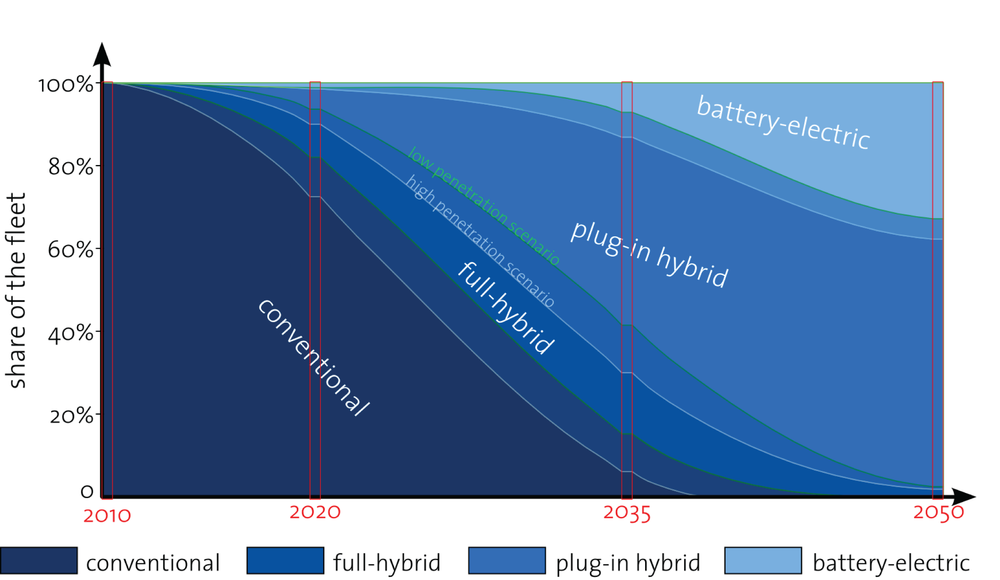
\includegraphics[width=0.65\textwidth, angle=0]{extending/figures/Elvehicles/main.png} \end{center}

\createStandardInformation{transEnergySim}{todo}{todo}{\citet[][]{WaraichEtAl_TRR_2013, GalusEtAl_STRC_2009, WaraichEtAl_IATBR_2009, GalusEtAl_ITSG_2012, Waraich_PhDThesis_2014, AbedinWaraich_TechRep_IVT_2013, WaraichEtAl_TechRep_IVT_2013, GalusEtAl_ResRep_EWZ_2012, Waraich_unpub_EURO_2012, Waraich_unpub_MATSimUserMeeting_2012, WaraichEtAl_JanssensEtAl_2014, WaraichAxhausen_SDEWES_2013}}

% ##################################################################################################################
\ah{can be deleted:

\begin{itemize}
	\item \lstinline|org.matsim.contrib.transEnergySim|
\end{itemize}

http://matsim.org/docs/extensions/transEnergySim

http://www.tesfw.org/
}

% ##################################################################################################################
\section{Electric Taxis} 
%\hfill \textbf{Author:} Joschka Bischoff\\
A combination and extension of both the TransEnergySim and the VRP contribution (see Chapter~\ref{ch:dts}) allows the simulation of taxi fleets constituting of battery electric vehicles (BEV).
On the electric vehicle side, charging process of vehicle is adapted, whereas on the taxi side the concept of taxi ranks and a modified optimizer that sends idling taxis to the rank and only dispatches vehicles with a sufficient battery state of charge are introduced. 

% ==============================================================================================
\subsection{Taxi Ranks}
After dropping off a passenger, taxis proceed to the nearest rank location, unless there is an immediate follow-up request. At the rank location a queuing takes place, i.e. the taxi that has arrived first will leave the rank the soonest. Other types of queuing have also been tested, e.g.,\,a dispatch by battery SOC.
Ranks are not necessarily mandatory, however driving to them in between trips resembles a typical taxi driver behavior in Germany.

% ==============================================================================================
\subsection{Charging Process}
Chargers may be located at taxi ranks or any other link. Following any given \lstinline$AgentArrivalEvent$ of a BEV at a charger location link, charging will commence if
%
\begin{itemize}
	\item There is a free charging spot
	\item The vehicle's SOC is under a certain threshold
	\item at least two minutes of time have passed that would be required for parking the car and plugging it in.
\end{itemize}

% ==============================================================================================
\subsection{Appliance}
So far, the simulation of electric taxis has been used in Mielec, Poland \citep[][]{Bischoff2013MaTaxis, BischoffMaciejewskiEcabMielecMobilTUM}. At the time of writing, an application for Berlin is in progress.

% ##################################################################################################################

